\documentclass[11pt]{article}
\usepackage[utf8]{inputenc}
\usepackage[T1]{fontenc}
\usepackage{amsmath}
\usepackage{amsfonts}
\usepackage{amssymb}
\usepackage[version=4]{mhchem}
\usepackage{stmaryrd}
\usepackage{graphicx}
\usepackage[export]{adjustbox}
\graphicspath{ {./images/} }

\begin{document}
Convertible Bond Arbitrage

The classic convertible bond arbitrage trade is to purchase a convertible bond that is believed to be undervalued and to hedge its risk using a short position in the underlying equity. The hedge is usually adjusted as the underlying stock rises or falls in value. If the underlying equity experiences volatility that is higher than the volatility implied by the original market price of the bond, then the strategy generates favorable returns. The convertible bond arbitrage strategy includes variations to the classic trade, such as using alternative hedging strategies, as well as to the reverse trade, involving a short position in a convertible bond perceived to be overvalued. Before discussing the actual trading strategy and describing its potential sources of return, we need to note the important characteristics of convertible bonds and explain the factors that affect the prices of these instruments.

\section*{Defining and Pricing Convertible Bonds}
Convertible bonds are hybrid corporate securities, mixing fixed-income and equity characteristics into one security. In their simplest form, convertible bonds can be thought of as a combination of an unsecured corporate bond and a call option on the issuer's stock. In a bankruptcy proceeding, convertible bonds are senior to equity securities and subordinated to senior and collateralized debt issues. The yield to maturity on convertible bonds is lower than the yield on otherwise equivalent straight debt because the convertible bond's conversion feature provides an option with substantial value to the holder. Because the holder of the convertible bond owns straight debt plus an equity call option, the owner is willing to pay a higher price (and accept a lower yield) than would be acceptable for an otherwise similar straight bond. Following are formulas for the value of a convertible bond, the conversion ratio, the option strike price, the conversion value, and the conversion premium of a convertible bond:

Thus, the firm in Application A can borrow $\$ 10$ million today in a bond issue and potentially never have to repay the loan in cash, as investors may opt to be repaid with 200,000 shares of stock at some date at or before the three-year maturity of the convertible bond. Valuing the convertible bond is typically accomplished by unbundling the structure into its component parts of straight debt and the equity call option, valuing each component, and summing their values.

In practice, convertible bonds are not valued by the Black-Scholes option pricing model that is used to value short-term equity options, as assumptions (including that of constant volatility) do not apply to long-dated convertible bond issues.

\section*{Busted, Hybrid, and Equity-Like Convertibles}
The characteristics of convertible bonds vary widely with the moneyness. Moneyness is the extent to which an option is in-the-money, at-the-money, or out-of-themoney. In the case of a convertible bond, moneyness indicates the relationship between the strike price implied by the conversion option and the price of the underlying stock. Bonds with very high conversion premiums (see Equation 1) are often called busted convertibles, as the embedded stock options are far out-of-themoney. These bonds behave like straight debt because when the stock option is far out-of-the-money, the convertible bond's value is primarily derived from its coupon and principal payments.

Bonds with very low conversion premiums have stock options that are deep in-the-money, where the convertible bond price and the conversion value are very close. The further in-the-money that the option is, the more the convertible bond behaves like the underlying stock. An equity-like convertible is a convertible bond that is far in-the-money and therefore has a price that tracks its underlying equity very closely. Interest rates and credit spreads matter less on equity-sensitive convertibles.

Convertible bonds with moderately sized conversion ratios have stock options closer to being at-the-money and are called hybrid convertibles. Hybrids are usually the most attractive bonds for use in convertible arbitrage strategies. These hybrid convertibles are attractive for convertible arbitrage due to their asymmetric payoff profile. The next exhibit illustrates the effect of moneyness on convertible bond prices and their sensitivity to the underlying equity prices. Note the convexity in the convertible bond price for hybrid convertibles. This convexity is the essential characteristic that drives the traditional convertible arbitrage strategy. The following section on delta, gamma, and theta provides a further foundation for understanding the dynamics of convertible arbitrage.

\begin{center}
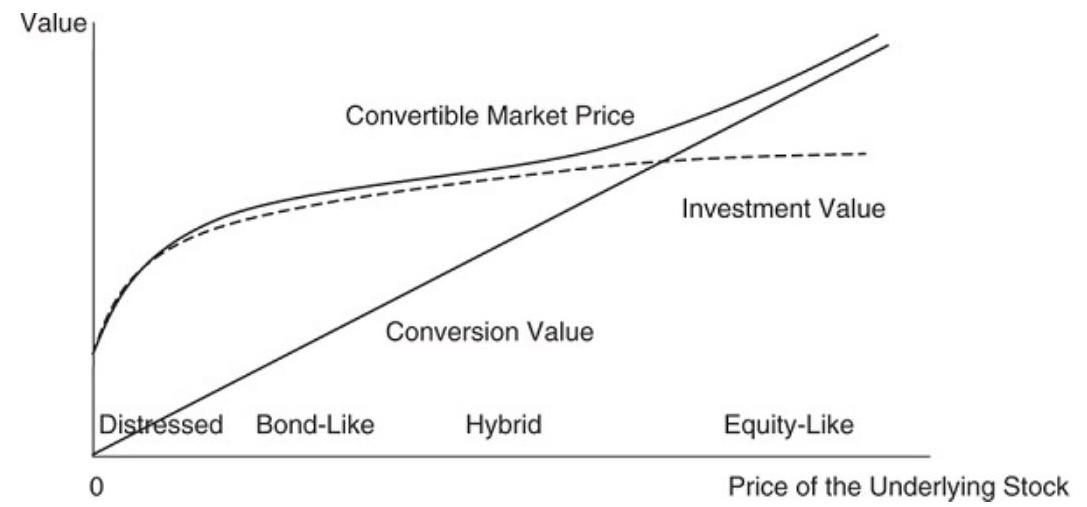
\includegraphics[max width=\textwidth]{2024_04_09_d2bdb6aa136bcf7c7f5eg-03}
\end{center}

Price Behavior of a Convertible Security

\section*{Delta, Gamma, and Theta}
The concepts of delta and gamma are keys to understanding the convertible arbitrage strategy. Delta is the change in the value of an option (or a security with an implicit option) with respect to a change in the value of the underlying asset (i.e., it measures the sensitivity of the option price to small changes in the price of its underlying asset). For example, if a $\$ 1$ rise in the value of a stock price causes a call option to rise $\$ 0.60$, then the delta of the call option is roughly $0.6 .{ }^{1}$ This relation holds only when there are very small changes in the value of the stock. Call options that are very far out-of-the-money have deltas near 0.0 , whereas options very far in-the-money have deltas near 1.0. The delta of a put option is negative. Delta is the first derivative of an option's price with respect to the price of the underlying asset and is a key concept in setting the hedge ratio of a convertible arbitrage position. In a graph of an option price against the price of the underlying asset, delta is the slope of the relationship at each point along the curve.

Gamma is the second derivative of an option's price with respect to the price of the underlying asset-or, equivalently, the first derivative of delta with respect to the price of the underlying asset. That is, it measures how delta changes as the price of the underlying asset changes. Graphically, gamma is the degree of curvature in the option price versus the underlying asset price relationship. Gamma measures the rate of change in the value of delta as the price of the underlying asset changes. Gamma is near zero when an option is extremely far out-of-the-money and the delta is very small. Gamma is also near zero when an option is extremely far in-themoney and the delta is near one. Gamma tends to be largest when the option is near-the-money. As illustrated in the next section, the gamma of a position can be used to describe how hedged positions earn money during periods of high volatility in the underlying asset.

Finally, theta is the first derivative of an option's price with respect to the time to expiration of the option. Theta is negative for a long position in an option, since as time passes and all other values remain the same, the option declines in value. In a nutshell, theta reflects the loss in an option's time value as time passes, which can be referred to as time decay. Theta is a key concept in understanding how hedged positions lose value if there are no changes in the underlying asset or its volatility. That is, theta is a cost to the buyer of the option and a benefit to the seller of the option, as the time value decays as the option approaches expiration. The goal of many active long-option trading strategies, including convertible bond arbitrage, is to earn sufficient profits from gamma trading to overcome the predictable losses from theta.

In summary, delta is used to establish the hedge ratio in a traditional convertible arbitrage position. The positive gamma or long gamma nature of the convertible bond ensures that the hedged position will make money if the underlying asset quickly rises or falls in value. This profit is generated by the unlimited upside and limited downside nature of a long position in an option (i.e., its curvature). Finally, the theta of the long option position indicates that as time passes, the hedged position loses value in the absence of underlying asset changes. Thus, a traditional convertible arbitrage strategy's return varies directly with the level of volatility experienced in the underlying asset. The goal in convertible arbitrage is to purchase undervalued options and short sell overvalued options while hedging other risks.

\section*{Stylized Illustration of Convertible Arbitrage}
Consider a $\$ 1,000$ face value convertible bond that can be converted into one share of stock, for mathematical simplicity. The stock currently sells for about $\$ 1,000$, so the implicit option is at-the-money. The next exhibit shows the five prices that the convertible bond can currently have for five possible stock prices. Notice that the convertible bond's price moves nonlinearly with respect to large changes in the underlying asset price, just like a call option does, with smaller losses to the downside and larger gains to the upside. This behavior is due to convexity and is a key to the profit potential.

\begin{center}
\begin{tabular}{lrrrrr|}
\hline
Stock Price & $\$ 960$ & $\$ 980$ & $\$ 1,000$ & $\$ 1,020$ & $\$ 1,040$ \\
Convertible bond price & $\$ 1,085$ & $\$ 1,090$ & $\$ 1,100$ & $\$ 1,110$ & $\$ 1,125$ \\
Long 1 bond and short 0.5 shares & $\$ 605$ & $\$ 600$ & $\$ 600$ & $\$ 600$ & $\$ 605$ \\
\hline
\end{tabular}
\end{center}

Assume that the current price of the stock is $\$ 1,000$ and the price of the convertible bond is $\$ 1,100$. If the stock rises or falls $\$ 20$, the convertible bond moves in the same direction but with half the magnitude (i.e., \$10). ${ }^{2}$ Technically speaking, the exhibit Example of a Delta-Neutral Position in Stocks and Convertible Bonds should not depict a linear relationship in the convertible bond for stock prices from $\$ 980$ to $\$ 1,020$, since the relationship is convex. The linearity was allowed to make computation of the delta more straightforward. The delta of the convertible bond is therefore 0.50 , and the hedged position would be a long position of one convertible bond and a short position of 0.5 shares of stock. The hedged position is said to be delta-neutral. A delta-neutral position is a position in which the valueweighted sum of all deltas of all positions equals zero. In this example, the sensitivity of the 0.5 short-sold shares to the equity price equals the sensitivity of one convertible bond to the equity price, offsetting each other and leaving the combined positions insensitive to small changes (i.e., a change of $\$ 20$ ) in the stock price.

The last line of the exhibit above illustrates that the hedged position breaks even for very small changes in the stock price; the combined positions retain a constant value of $\$ 600$. But the combined positions are profitable for either a $\$ 40$ up or a $\$ 40$ down movement in the underlying asset. This illustrates that even though the positions are delta-neutral, the hedge benefits from large movements in either direction. The profit is generated by the positive gamma of the convertible bond, wherein losses of the bond slow down when the stock declines, and profits accelerate when the stock rises. If a large price change in the underlying asset takes place, the hedged position makes a profit, and the positions are adjusted to being delta-neutral based on a new hedge ratio at the new price levels. If the underlying stock price does not move, the convertible bond will slowly decline to its par value at maturity, and the hedged position will fall to $\$ 500$, illustrating the negative theta.

In a convertible arbitrage strategy, when the underlying stock price has changed and the positions (i.e., the hedge ratio) have been adjusted to bring the exposure back to being delta-neutral, it does not matter whether the stock price moves back to its original value or continues moving in the same direction. The reason it does not matter is that once the stock price has changed and the arbitrageur has reset the hedge to reflect the new hedge ratio by expanding or contracting the short position in the stock, the positions are returned to being delta-neutral. Once the positions are returned to delta neutrality, the positions return to the profit and loss exposures illustrated in the exhibit above and the arbitrageur returns to being able to profit whether the next move in the stock is up or down.

Note, however, that for the arbitrageur to make more money on gamma than is being lost on theta, which is known as time decay, the stock must keep experiencing substantial price changes. These price changes dictate the relationship between realized volatility and implied volatility. Realized volatility is the actual observed volatility (i.e., the standard deviation of returns) experienced by an asset-in this case, the underlying stock. The implied volatility of an option or an option-like position-in this case, the implied volatility of a convertible bond-is the standard deviation of returns that is viewed as being consistent with an observed market price for the option. A traditional convertible arbitrage strategy is a play on whether the realized volatility is equal to, less than, or greater than the implied volatility of the convertible bond price when the position was established. The keys to convertible arbitrage success are to buy convertible bonds with underpriced conversion options (i.e., implied volatility that is too low), short sell convertible bonds with overpriced conversion options (i.e., implied volatility that is too high), and maintain hedges by taking offsetting positions in the underlying equity to control for risk. By far the most common strategy is to take a long position in the convertible bond and hedge the market risk of the position by taking a short position in the underlying equity. Fund managers who follow this strategy believe that the implied volatilities of convertibles are too low when compared to the expected realized volatility of the stock.

\section*{Convertible Arbitrage and Short Selling}
The most common convertible arbitrage strategy involves short selling large quantities of the common stock underlying the convertible bond's embedded option. As detailed in Session 2.2, The Environment of Alternative Investments, the steps in selling assets short include the following:

\begin{enumerate}
  \item Borrowing the assets from an entity that currently owns them. There is an active market between entities that borrow assets and entities that lend assets, known as securities lending. Securities lending is generally facilitated by an intermediary, usually an investment bank or a brokerage firm.

  \item Selling the borrowed assets into the market.

  \item Eventually closing the position by purchasing the assets from the market and delivering them to the entity from which they were borrowed.

\end{enumerate}

\section*{Convertible Bond Arbitrage Background}
Convertible bond arbitrage offers the potential to earn alpha when the options implicit in the bonds are mispriced. Why might convertible bond prices be attractive? As a small and complex asset class, convertible bonds may offer liquidity or complexity premiums to skilled hedge fund managers who are able to evaluate them and identify the potential mispricing that results from their complexity. A complexity premium is a higher expected return offered by a security to an investor to compensate for analyzing and managing a position that requires added time and expertise. Convertible bonds, already made complex by the conversion options, become especially complex when the bonds stray from the plain-vanilla package of corporate debt plus a conversion option to having the additional complexities of callable or putable convertibles, dual currencies, and/or forced conversions.

Convertible bond arbitrage funds develop computerized systems to scan the universe of convertible bonds and compare convertible bond prices to the price of the straight debt and equity call option package. Each hedge fund creates customized assumptions for the straight bond yield and the volatility of the underlying equities. The analysis of the underlying straight bond focuses on the firm's credit risk, whereas the analysis of the equity volatility focuses on historical return volatilities and current option prices. When the convertible bond is undervalued relative to the sum of its parts, the hedge fund purchases the convertible bond and shorts the underlying equity. Less often, the convertible bond is viewed as overvalued and sold short with a long position in the underlying equity. Also, the convertible bond position is sometimes hedged with positions in equity options in addition to or in place of positions in equities. Further, to hedge the interest rate risk and credit risk of the convertible bonds, the manager sometimes establishes positions in interest rate derivatives or credit derivatives.

\section*{Four Sources of Returns to Convertible Bond Arbitrage}
Fund managers who are able to develop accurate predictions of equity volatility relative to the volatility implied by convertible bond prices can earn superior returns by buying undervalued convertible bonds and shorting the underlying equity. In the past two decades, convertible bond arbitrage trading tended to focus on long\\
positions in convertible bonds and to generate superior returns, especially in the mid- to late 1990s, indicating that convertible bonds themselves offered consistently superior returns.

Note, however, that if investors in convertible bonds consistently earned superior returns, the bonds might offer higher than necessary yields, which make convertible bonds an expensive source of corporate financing (i.e., the return earned by the bond investor is the cost of capital to the firm). In perfect capital markets, the risk-adjusted costs of all sources of financing would be forced toward equality, since investors would avoid buying securities with returns too low and corporations would avoid issuing securities with returns too high. There are two elements necessary to support the argument that convertible bonds should consistently offer superior risk-adjusted returns. First, demand to buy convertible bonds must be restricted such that it prevents convertible bond prices from increasing to the point of offering normal risk-adjusted returns. Second, suppliers of convertible bonds (corporations) must be of sufficient size to suppress convertible bond prices to the point of allowing superior returns.

The argument that there is limited demand from convertible bond investors appears plausible. The complexity of convertible bond analysis and hedging, combined with restrictions on the ability of traditional investment managers such as mutual fund managers to short equity, may limit the number of investors willing and able to perform convertible bond arbitrage. But why would corporations issue convertible bonds if they were consistently underpriced? More broadly, are there solid reasons to believe that convertible bonds will continue to be issued at prices that offer consistently high risk-adjusted returns to investors and therefore higher costs to issuers? There are four especially persuasive reasons to believe that issuers may, at least periodically, continue to offer convertible bonds at attractive prices:

\begin{enumerate}
  \item Agents (corporate managers) may underestimate the true costs of issuing convertible bonds. Convertible bonds offer yields that substantially underestimate expected returns when those yields are based on coupons and principal amounts. Issuers may find the lower yields to be attractive, as the coupon interest rate on convertible bonds is lower than the interest rate paid on the straight bonds issued by the firm. The issuers may not fully appreciate the potential harm to share prices from dilution when the implicit options are exercised. Dilution takes place when additional equity is issued at below-market values, and the pershare value of the holdings of existing shareholders is diminished.

  \item Agents of small firms may have no choice but to issue convertible bonds at attractive prices. Convertible bonds are rarely registered in a public offering. In the United States, most convertible bonds are sold as 144A exempt securities, meaning they are exempt from the registration requirements of the SEC (Securities and Exchange Commission). As a result, most convertible bonds cannot be sold to retail investors, and trade only among institutional investors. The lack of a public market for these convertible bonds makes them less liquid than stocks or regular bonds. Consequently, their prices may be lower and their returns higher as a premium for bearing liquidity risk.

  \item There is a potentially substantial conflict of interest between straight bond investors and shareholders with regard to preferred corporate asset volatility. Straight bondholders prefer low asset volatility to decrease the probability of bankruptcy. Equity holders have a risk exposure that can be viewed as a call option on the firm's assets, and, therefore, they may prefer high asset volatility. Shareholders have an incentive to increase the volatility of the firm's assets after the issuance of debt, in order to transfer wealth from bondholders to themselves. Since bondholders are aware of this potential risk, they demand a higher yield for compensation, and suboptimal corporate investment decisions may result. The incentive to take on excessive risk is reduced if convertible bonds are issued, as any increase in volatility benefits the convertible bondholders as well as the equity holders. In short, convertible bonds reduce agency costs and lead to a lower cost of capital for the firm. Asymmetric information between corporate managers and investors regarding asset volatility can exacerbate the problems with issuing straight debt. Since convertible bonds are hybrid investments, their prices are less sensitive to the credit risk of the issuing firm. This insensitivity makes it easier for the firm and potential bondholders to agree on the value of the bond when convertible debt is used and there is substantial uncertainty about the riskiness of corporate assets.

  \item Indirect equity issuance costs are a factor. Corporations use convertible bonds as an indirect way to issue equity because their cost of directly issuing new equity may be high. For instance, when managers opt to issue new stock at current price levels, potential buyers of the new shares may conclude that managers and current shareholders view the current price as being above its fair value, making them willing to bring in new investors. The inadvertent information signal caused by issuing equity could depress share prices as market participants react to the concern that the firm is in worse financial condition than originally believed and as reflected in the share price. Since most convertibles are converted into equity only if the stock price increases, the signal conveyed to the market is not viewed as negatively as when equity is issued.

\end{enumerate}

\section*{Components of Convertible Arbitrage Returns}
The components of convertible arbitrage returns include interest, dividends, rebates, and capital gains and losses. The next exhibit depicts these components for the case of a traditional convertible bond strategy of being long the convertible bond and short the underlying stock. The first component of the return of a traditional convertible arbitrage strategy is the income component. Assuming a long position in the convertible bond and a short position in the stock, the investor earns the coupon interest paid on the bond, pays any dividends due on the short stock position, and earns a rebate on the cash proceeds from the short sale of the stock. If there are any costs to financing the position, such as the cost to borrow the stock or the interest paid on leveraged positions, those costs are deducted from the arbitrage income.

\begin{center}
\begin{tabular}{c}
Components of the Return of a Traditional Convertible Arbitrage Strategy \\
Convertible Bond Arbitrage Income = \\
(Bond Interest - Stock Dividends + Short Stock Rebate - Financing Expenses) \\
\hline
+ \\
(Capital Gains on Stock and Bond - Capital Losses on Stock and Bond) \\
\end{tabular}
\end{center}

The second source of the return to the convertible bond arbitrageur is the gain on stock trading (and, to a lesser extent, the possible gain or loss on the eventual sale of the convertible bond), as illustrated in the exhibits Example of a Delta-Neutral Position in Stocks and Convertible Bonds, and Components of the Return of a Traditional Convertible Arbitrage Strategy. In the traditional convertible arbitrage trade of being long the convertible bond, the larger and more frequent the stock price moves, the greater the profits from gamma trading. Profits from gamma trading, though, are offset through theta, or time decay. The goal of gamma trading is to earn more in profits from gamma than the option value loses in time decay. This goal is met when the realized volatility of the stock exceeds the implied volatility priced into the option on the day the convertible bond is purchased.

This simplified discussion of convertible arbitrage has held constant other sources of risk and return, such as interest rates, credit spreads, and implied volatility. Although some convertible bond managers are content to maintain a simple hedge of the convertible bond against the underlying stock, other managers may seek to\\
hedge other risks or add further value through derivative strategies related to interest rates, credit spreads, volatility, or stock price anticipation. For example, more sophisticated hedging strategies use interest rate and credit derivatives to hedge interest rate and credit spread risks such that the arbitrage is more of a pure play on realized volatility relative to implied volatility.

Some convertible arbitrage hedge funds attempt to identify and hedge the underpriced embedded options of a convertible bond by buying the convertible bond and selling short an exchange-traded call option on the underlying stock. This technique can be effective when there is a large spread in implied volatility between exchange-traded and embedded call options. However, there is rarely a clean match between listed and embedded options in terms of exercise periods, and many convertible bond issuers do not have options listed on their stock. Interest rate hedges are less common in convertible arbitrage funds. Given that much of the convertible bond universe is below investment grade, credit spread changes can be significantly more important than changes in risk-free or investment-grade interest rates. Credit derivatives, detailed in Session 6.2, Credit Risk and Credit Derivatives, can be useful vehicles with which to hedge credit risk.

Rather than hedging various risk exposures, managers may speculate on them. Profits from a convertible arbitrage position can be substantially enhanced when managers have the ability to consistently predict the future path of interest rates, credit spreads, stock prices, or volatility. For example, to add value through credit spread anticipation, the manager may perform fundamental credit analysis on each issuer, seeking to purchase bonds with improving credit quality and tightening credit spreads, while avoiding bonds whose credit quality is deteriorating, which can lead to widening credit spreads. For stock price anticipation, the manager deviates from delta neutrality in an attempt to profit from stock price moves in a particular direction. The manager applies heavy delta hedges (a net short position) to stocks expected to underperform, and light delta hedges (a net long position) to stocks for which higher prices are anticipated. Fund managers are also likely to diversify their portfolios across issuer, sector, maturity, and so forth to reduce both idiosyncratic risk and exposures to industries and sectors.

\section*{Details Regarding Convertible Bond Arbitrage}
Let's take a close look at how a traditional convertible arbitrage strategy tries to enhance returns. Specifically, this section details how a position that is delta hedged can earn gains from gamma (convexity) that more than offset the losses from theta (time decay).

Delta hedging is shown in this example to reduce risk; however, delta hedging does not eliminate the potential for net capital gains. Due to the nonlinear nature of their payoff, most at-the-money convertible bonds exhibit a desirable property known as positive convexity, or high gamma. That is, they appreciate in value from an immediate upward stock price change more than they depreciate from the same sized downward change in the underlying stock price. This section shows that a delta-hedged position will actually benefit from any movement in the underlying stock due to this convexity. The traditional arbitrage strategy speculates that there will be enough movements in the stock price (i.e., volatility) to generate gains from gamma that more than offset the losses from theta (the time decay of the position).

Consider an example of convertible bond XYZ with a conversion ratio of 8. A convertible bond arbitrageur believes that the implicit option in the bond is undervalued and that therefore the entire bond is underpriced based on the arbitrageur's estimate of the future volatility of the underlying asset (stock). How can the arbitrageur exploit such a mispricing? Buying the cheap convertible bond is clearly part of the solution, but it is not sufficient. Simply waiting for market prices to adjust is not an arbitrage because the long convertible position comes with a variety of risks that could easily wipe out the expected gains. To arbitrage, it is necessary to both buy the cheap convertible bond and hedge its risks, a dynamic process that is very similar to what arbitrageurs of listed options do on a regular basis.

The primary risk of holding a long convertible position comes from the potential variations in the underlying stock price. This equity risk can be easily eliminated by selling short an appropriate quantity of the underlying stock. This quantity corresponds to the convertible's delta multiplied by the number of shares into which the bond may be converted. Let's assume that the delta of the XYZ convertible bond is 0.625 . To hedge the equity risk, an arbitrageur would need to sell short delta times the conversion ratio $(0.625 \times 8=5.0)$ shares of stock per $\$ 1,000$ face value of the convertible bond bought. If the stock price gains $\$ 1$, the convertible bond will gain approximately delta (times 8) dollars and the short stock position will lose delta (times 8) dollars, so that the overall variation will be near zero. Conversely, if the stock price drops by $\$ 1$, the convertible bond will lose approximately the same number of dollars that the short stock position will gain. As illustrated in Delta Hedging a Convertible Bond, for a small change in the price of the stock, the arbitrageur's position will be hedged.

\begin{center}
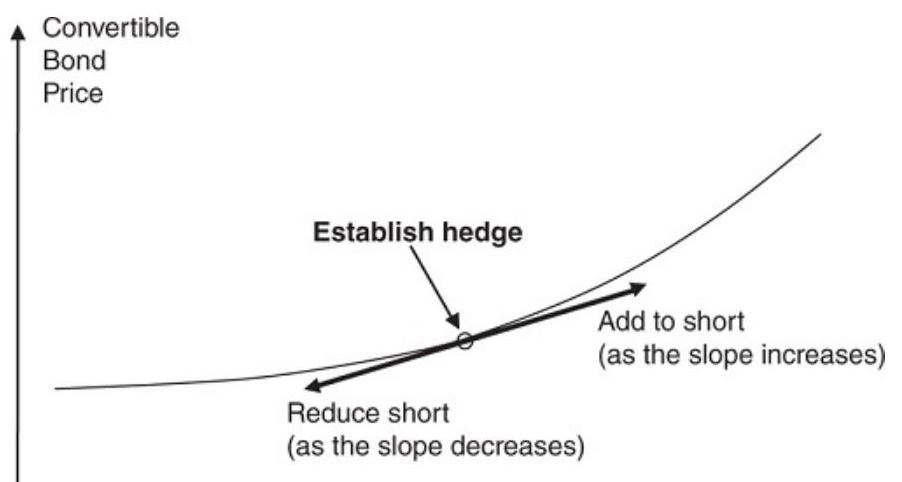
\includegraphics[max width=\textwidth]{2024_04_09_d2bdb6aa136bcf7c7f5eg-06}
\end{center}

Stock Price

\section*{Delta Hedging a Convertible Bond}
But this approximation ignores a key aspect to the hedge: Although delta hedging reduces the risk from changes in the underlying stock price, it does not eliminate return. Return of the strategy can be enhanced because, ignoring theta, the hedged position generates a small gain whether the underlying stock moves up or down, due to the position's gamma. This important concept is detailed later.

First let's focus on the need to rebalance the original delta-hedged position. In our example, when the stock price changes, the delta of the convertible bond will no longer be 0.625 , and, therefore, the net delta of the position will no longer be equal to zero. The net delta of a position is the delta of long positions minus the delta of short positions.

As the stock price increases, the option component moves further in-the-money and the convertible bond becomes more equity sensitive (see the exhibit Delta Hedging a Convertible Bond). The delta of the convertible bond increases, so the arbitrageur must adjust the hedge by shorting more shares. Conversely, as the stock\\
price declines, the option moves out-of-the-money, the delta of the convertible bond declines, and the arbitrageur must reduce the hedge by buying back some shares.

For example, if the delta rises to 0.70 due to a stock price increase, the short position must be expanded from 5.0 shares to 5.6 shares ( $8 \times 0.70$ ). If the delta falls to 0.50 due to a stock price decrease, the short position must be contracted to 4.0 shares $(8 \times 0.50)$. The hedge needs to be rebalanced repeatedly as the stock price moves, in a strategy known as dynamic delta hedging. Dynamic delta hedging is the process of frequently adjusting positions in order to maintain a target exposure to delta, often delta neutrality.

A key question for most arbitrageurs is how often they should rebalance their hedges. Arbitrageurs usually rehedge based on a time or price formula. In the former case, rehedging takes place at prespecified time intervals, such as every day or every hour. In the latter case, rehedging takes place whenever the stock price changes by a certain amount (e.g., every $\$ 1$ move or every $1 \%$ move in the stock price) or when the size of the necessary adjustment reaches a certain threshold.

Let's look more closely at the convexity, or gamma, that drives the traditional convertible bond arbitrage strategy. Gamma refers to the asymmetric valuation profile generated by movements in the underlying stock price. In other words, gamma is illustrated by the curvature in the next exhibit.

\begin{center}
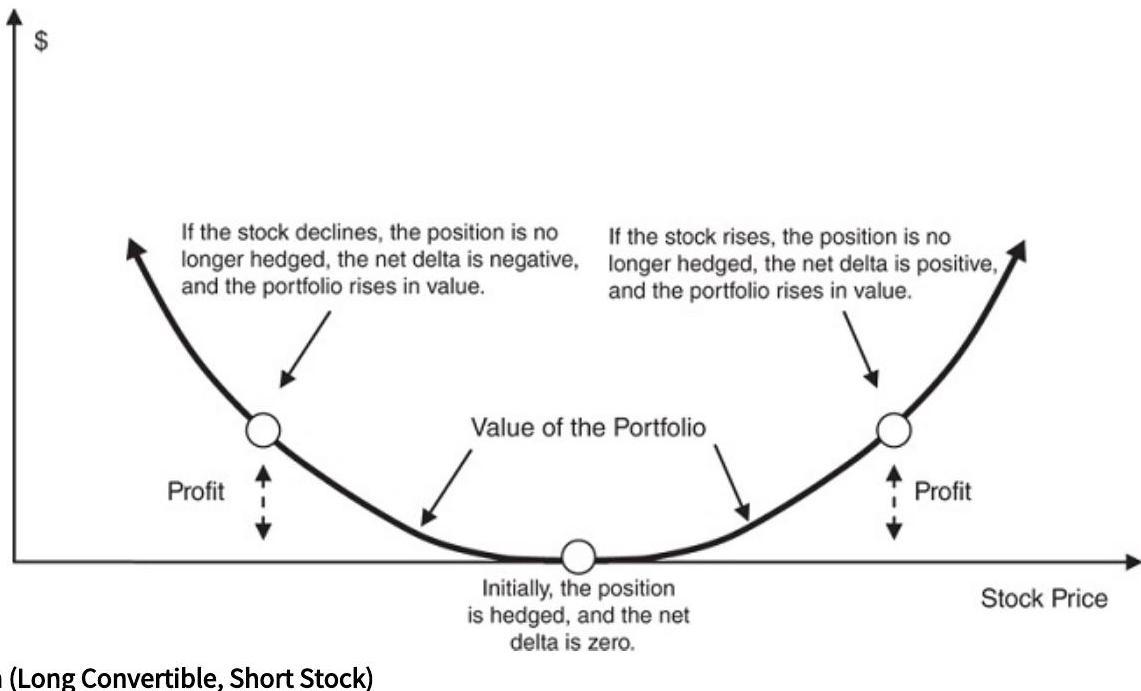
\includegraphics[max width=\textwidth]{2024_04_09_d2bdb6aa136bcf7c7f5eg-07}
\end{center}

The exhibit above illustrates why the gamma of the convertible bond generates a gain to the hedged position when the underlying stock moves up or down. But the Profit on a Delta-Hedged Position (Long Convertible, Short Stock) exhibit does not illustrate the downside risk. The worst outcome for the traditional convertible bond arbitrageur is when the stock price remains unchanged. When the stock price does not change, the hedged position loses value due to the theta (time decay) of the long position in the implicit option. When the underlying stock price experiences less volatility than is implied by the bond price, the losses from the theta of the option more than offset the gains from the gamma, and the strategy underperforms.

Saying that a convertible bond is cheap is equivalent to saying that the corresponding implied volatility is too low. If realized volatility is higher than implied volatility, then the profits illustrated in the exhibit above should dominate the theta, resulting in net profits for the strategy. Conversely, if the realized volatility is below the implied volatility, the loss due to theta will outweigh the profit made from the realized volatility, and the position will underperform a risk-free investment, perhaps even incurring a loss.

\section*{Return Drivers of Convertible Bond Arbitrage}
The mispricing of convertible bonds can be relatively large or small. Minor differences in the volatility used to price the embedded stock option in a convertible bond can generate substantial price differences. For example, if a three-year convertible bond is mispriced by two volatility points (e.g., $25 \%$ volatility is used to price the bond rather than $27 \%$ ), the convertible bond may be underpriced by $1 \%$, a mispricing that may take three years to fully correct. In cases of small degrees of mispricing, convertible bond arbitrage hedge funds may apply leverage to increase the expected returns. Before the 2008 financial crisis, it was not uncommon to see convertible bond hedge funds trade at leverage of over eight times investor capital. Since 2008, it has become more difficult to leverage positions, with the result that some convertible bond funds may now forgo leverage, while others may be able to reach a maximum leverage of only four times investor capital.

It is easy to see why hedge fund managers are tempted to use leverage, as they earn incentive fees on each additional dollar of returns they earn. But leverage is a two-edged sword to investors, as it magnifies both gains and losses. However, incentive fee-based hedge fund managers disproportionately participate in the gains but not the losses; thus, as detailed in Session 5.1, Structure of the Hedge Fund Industry, the managers may increase the value of their incentive fee option by taking larger risks.

The market crisis of 2008 created unprecedented risks and opportunities for convertible bond arbitrage. The Credit Suisse Convertible Bond Arbitrage Index declined by more than $25 \%$ during the last four months of 2008. This decline may have been caused by illiquidity and large amounts of forced selling of convertible bonds, as prime brokers forcibly reduced the availability of leverage, and the large portfolio of the now-defunct Lehman Brothers was quickly sold into the market. Once this selling subsided, the opportunities in the convertible bond market were unprecedented, as mispricing reached record levels. The yield on US investment-grade convertible bonds reached $14.9 \%$ in March 2009, wider than the straight bond yield of $11.0 \%$ of the same issuers. A convertible bond arbitrage fund could apparently buy the convertible bond and sell short the straight bond of the same issuer, receiving a free option and an extra yield of $3.9 \%$. Summary of Convertible Bond Arbitrage Risks summarizes the risks of convertible bond arbitrage.

Summary of Convertible Bond Arbitrage Risks

\begin{center}
\begin{tabular}{|lll|}
\hline
Risk & Position & Effect \\
\hline
Interest rates & \begin{tabular}{l}
Long convertible bond, long \\
duration, long convexity \\
\end{tabular} & \begin{tabular}{l}
Convertible bonds have an exposure to risk-free interest rates. As rates rise, bond prices fall. Some funds \\
hedge these risks through the use of sovereign bond futures or interest rate swaps. \\
\end{tabular} \\
\hline
\end{tabular}
\end{center}

\begin{center}
\begin{tabular}{|c|c|c|}
\hline
Risk & Position & Effect \\
\hline
\begin{tabular}{l}
Equity and \\
volatility \\
\end{tabular} & \begin{tabular}{l}
Short stock, delta-neutral, \\
long gamma, long vega, long \\
theta \\
\end{tabular} & \begin{tabular}{l}
When the convertible bond arbitrage manager takes a short equity position of the appropriate size, the \\
equity risk of the convertible bond is hedged. The embedded long positions in vega and gamma can \\
increase profits when volatility rises. However, the passage of time works against the investor, as the \\
option's time value, measured by theta, decays over time. \\
\end{tabular} \\
\hline
Correlation & Long bond-equity correlation & \begin{tabular}{l}
The strategy is long correlation: When interest rates rise, losses may be offset by gains on the short equity \\
positions. When interest rates fall, losses on the short equity position offset the fixed-income gains. When \\
correlation declines, stock and bond prices move in opposite directions, causing losses on both \\
components of the convertible bond. \\
\end{tabular} \\
\hline
Credit & Long convertible, short equity & \begin{tabular}{l}
Convertible bonds have an exposure to credit risk. As credit spreads widen, bond prices fall. All bonds have \\
a senior claim relative to equities during bankruptcy proceedings. \\
\end{tabular} \\
\hline
Legal & Long convertible & \begin{tabular}{l}
Adverse regulatory rulings can negatively affect convertible bond arbitrageurs. Reductions in leverage \\
ratios, short-selling restrictions, and accounting changes that make convertible issuance more restrictive \\
can cause unexpected losses for arbitrageurs. \\
\end{tabular} \\
\hline
\begin{tabular}{l}
Liquidity and \\
crisis \\
\end{tabular} & Short equity, long convertible & \begin{tabular}{l}
Convertible bond investors sell economic disaster insurance as credit spreads widen during times of \\
economic crisis. Convertible bond arbitrageurs are exposed to liquidity risks, such as equity short \\
squeezes, widening bid-ask spreads of convertible bonds, and increases in both the short stock borrowing \\
rate and the prime broker borrowing rate. \\
\end{tabular} \\
\hline
\end{tabular}
\end{center}

Adapted from Alexander Ineichen (2003), Absolute Returns (Hoboken, NJ: John Wiley \& Sons).

\section*{Key Observations Regarding Historical Returns of Convertible Arbitrage Funds}
Monthly returns to convertible arbitrage hedge funds are observed from January of 2000 to December of 2021, for a total of 264 observations. Statistical Summary of Returns provides univariate return statistics and partial autocorrelations of returns in the top panel, and histograms of returns in the bottom panels.

\begin{center}
\begin{tabular}{lcc}
\hline
\begin{tabular}{c}
Index (Jan. 2000- \\
Dec. 2021) \\
\end{tabular} & \begin{tabular}{c}
HFRI Relative Value: Fixed \\
Income-Convertible \\
Arbitrage Index \\
\end{tabular} & \begin{tabular}{c}
MSCI Worid \\
Equity \\
\end{tabular} \\
\hline
Annualized Arithmetic Mean & $6.3 \%$ & $6.8 \%$ \\
Annualized Standard Deviation & $6.9 \%$ & $15.4 \%$ \\
Annualized Semivolatility & $7.2 \%$ & $11.8 \%$ \\
Annualized Median & $8.0 \%$ & $15.1 \%$ \\
Skewness & -2.8 & -0.6 \\
Excess Kurtosis & 25.1 & 1.6 \\
Sharpe Ratio & 0.5 & 0.3 \\
Sortino Ratio & 0.5 & 0.4 \\
Annualized Geometric mean & $6.1 \%$ & $5.6 \%$ \\
First-Order Autocorrelation & 0.5 & 0.1 \\
Annualized Standard Deviation & $12.2 \%$ & $17.0 \%$ \\
(Adjusted for Autocorrelation) & $9.7 \%$ & $12.8 \%$ \\
Maximum & $-16.0 \%$ & $-19.0 \%$ \\
Minimum & $-35.3 \%$ & $-54.0 \%$ \\
Max Drawdown &  &  \\
\hline
 &  &  \\
 & HFRI Relative & MSCI Worid \\
Index (Jan. 2000- & Value (Total) & Equity \\
Dec. 2021) & $6.1 \%$ & $6.8 \%$ \\
Annualized Arithmetic Mean & $4.5 \%$ & $15.4 \%$ \\
Annualized Standard Deviation & $5.0 \%$ & $11.8 \%$ \\
Annualized Semivolatility & $7.4 \%$ & $15.1 \%$ \\
Annualized Median & -3.5 & -0.6 \\
Skewness & 23.3 & 1.6 \\
Excess Kurtosis & 0.8 & 0.3 \\
Sharpe Ratio & 0.7 & 0.4 \\
Sortino Ratio & $6.0 \%$ & $5.6 \%$ \\
Annualized Geometric mean & 0.2 & 0.0 \\
First-Order Autocorrelation & $6.7 \%$ & $17.0 \%$ \\
Annualized Standard Deviation & $3.9 \%$ & $12.8 \%$ \\
(Adjusted for Autocorrelation) & $-9.8 \%$ & $-19.0 \%$ \\
Maximum & $-18.0 \%$ & $-54.0 \%$ \\
Minimum &  &  \\
Max Drawdown &  &  \\
\hline
\end{tabular}
\end{center}

PARTIAL AUTOCORRELATION FUNCTION FOR HFRI RELATIVE VALUE:\\
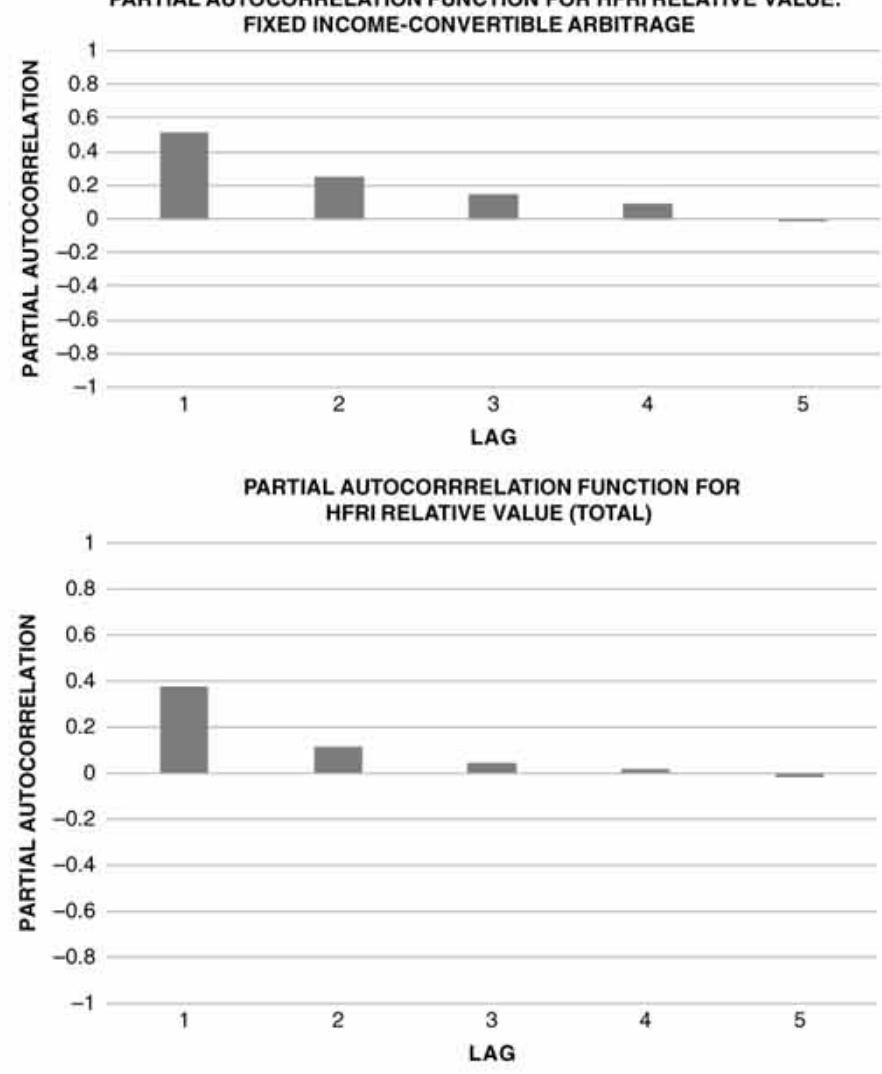
\includegraphics[max width=\textwidth, center]{2024_04_09_d2bdb6aa136bcf7c7f5eg-09}

Histogram of HFRI Relative Value: Fixed Income-Convertible Arbitrage Returns (Monthly) Jan. 2000-Dec. 2021

\begin{center}
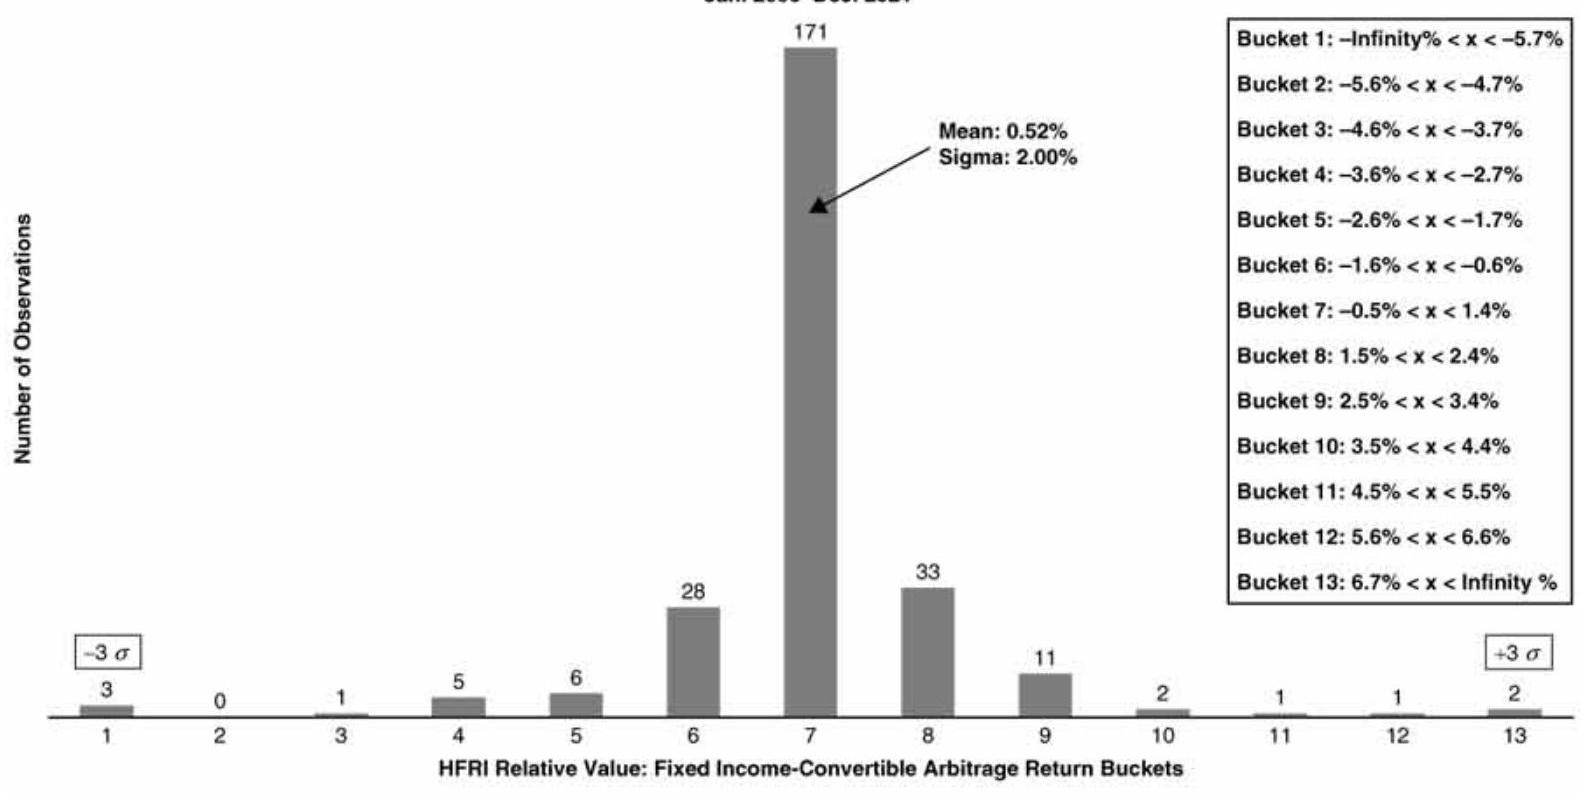
\includegraphics[max width=\textwidth]{2024_04_09_d2bdb6aa136bcf7c7f5eg-09(1)}
\end{center}

Histogram of HFRI Relative Value (Total) Returns (Monthly) Jan. 2000-Dec. 2021

Bucket 1: -Infinity\% $1 x<-3.1 \%$\\
Bucket 2: $-3.0 \%<x<-2.5 \%$\\
Bucket 3: $-2.4 \%<x<-1.9 \%$\\
Bucket 4: $-1.8 \%<x<-1.3 \%$\\
Bucket 5: $-1.2 \%<x<-0.7 \%$\\
Bucket 6: $-0.6 \%<x<-0.2 \%$\\
Bucket 7: $-0.1 \%<x<1.0 \%$\\
Bucket 8: 1.1\%<x<1.6\%\\
Bucket 9: 1.7\%<x<2.1\%\\
Bucket 10: $2.2 \%<x<2.8 \%$\\
Bucket 11: $2.9 \%<x<3.3 \%$

\section*{Statistical Summary of Returns}
Key observations on convertible arbitrage returns that are consistent with economic reasoning are an essential component of knowledge and include the following:

\begin{enumerate}
  \item The historical return distribution of convertible arbitrage exhibited moderately greater left skew and extraordinarily high excess kurtosis relative to global equities.

  \item Volatility of returns was moderately lower than that of world equities.

  \item Returns exhibited strong positive first-order autocorrelation.

  \item Maximum drawdown was moderately milder than observed for global equities.

\end{enumerate}

\end{document}